\label{chap:07_domain_adaptation}
\newcommand{\deacc}[0]{\textbf{deacc}}
\newcommand{\cased}[0]{\textbf{cased}}
\newcommand{\uncased}[0]{\textbf{uncased}}

En este capítulo analizaremos cómo mejorar la detección de discurso de odio desde una perspectiva más general, centrándonos en aplicar técnicas de \textbf{adaptación de dominio} a los algoritmos de clasificación que han sido considerados hasta el momento. Como hemos mencionado en la Sección \ref{sec:03_preprocessing}, cuando hablamos de adaptación de dominio nos referimos al el conjunto de técnicas y recursos destinados a tratar de que los algoritmos tengan un correcto desempeño en un subconjunto de tareas relacionadas entre sí \cite{goodfellow2016deep}. En el caso concreto de las tareas cuyas instancias constan de analizar texto de usuarios en redes sociales u otros medios, \citet{eisenstein2013bad} describió a la adaptación de dominio en términos de la necesidad de construir herramientas propias para este tipo de texto, muy distinto al lenguaje formal proveniente de otras fuentes.

Las técnicas de representación modernas --desde los embeddings hasta los modelos de lenguaje-- suelen ser entrenadas sobre conjuntos de datos que se suponen lo suficientemente generales. Fuentes usuales son Wikipedia, que comprende textos de carácter enciclopédico, o Common Crawl, que es una recopilación de datos de distintos sitios web. El uso del lenguaje en estas fuentes suele guardar una considerable discordancia con el de muchas tareas de interés en NLP, como son aquellas basadas en textos provenientes de ciertos nichos donde el uso del lenguaje es muy específico. Ejemplos de esto son los documentos médicos, trabajos científicos, entre otros. A cada uno de estos grupos de textos con cierta relación se los denomina --de manera poco precisa-- \textbf{dominios}. Entre estos, el contenido informal de las redes sociales tiene variedades lingüísticas muy particulares, con mucha jerga, expresiones coloquiales, errores ortográficos y demás que diferencian el uso del lenguaje de los textos fuentes mencionados.

Continuamos en este Capítulo alguna de las ideas y observaciones que hemos analizado previamente acerca de la adaptación de dominio. En primer lugar, en el Capítulo \ref{chap:03_social_text_classification} se ha observado que las técnicas de representación --desde los word-embeddings hasta los modelos de lenguajes-- tienen un buen desempeño sobre tareas de textos de redes sociales son entrenadas sobre este mismo dominio. Para el idioma español, sin embargo, no existe ningún modelo de lenguaje fácilmente accesible de estas características, como BERTweet para el inglés o AlBERTo en italiano. Describimos entonces el proceso de entrenamiento desde cero de un modelo de lenguaje sobre tweets en español, al cual llamamos \robertuito{}. Evaluamos su rendimiento compilando todas las tareas analizadas en esta tesis, y mostramos que es superior a todos los modelos considerados hasta el momento.

En segundo lugar, retomaremos otro enfoque para adaptar las técnicas existentes al dominio de redes sociales. En el Capítulo \ref{chap:06_contextualized_hate_speech} conseguimos mejorar la performance de los algoritmos de clasificación mediante la continuación del pre-entrenamiento del modelo de lenguaje sobre un gran conjunto de datos de noticias y comentarios no etiquetados, los cuales fueron recolectados como parte del proceso de construcción del dataset usado. Trabajo reciente muestra que esta técnica es generalizable a muchos dominios --como textos médicos, científicos, entre otros-- y resulta en mejoras consistentes del rendimiento de los algoritmos de clasificación basados en \bert{} y similares. En nuestro caso, analizaremos el efecto de continuar el pre-entrenamiento ya no sólo sobre la tarea de detección contextualizada de discurso de odio sino sobre todas las tareas que hemos visto en los diferentes capítulos.

Finalmente, haremos una comparación entre estas dos aproximaciones a adaptar nuestros algoritmos a este medio, algo de lo que no tenemos conocimiento se haya realizado hasta el momento, al menos para el idioma español. Este punto es de interés dado el gran costo que tiene entrenar modelos basados en Transformers, y sirve para verificar si el salto en el rendimiento de los modelos generados para dominios específicos puede subsanarse mediante una alternativa más económica como es la continuación del pre-entrenamiento.

Comenzamos en la Sección \ref{sec:domain_adaptation_previous_work} haciendo un racconto de las técnicas de adaptación de dominio y modelos pre-entrenados. Describimos a continuación la  construcción y el entrenamiento de \robertuito{} \cite{perez2021robertuito}. Finalmente, detallamos los experimentos de adaptación utilizando \beto{} como modelo de lenguaje a adaptar para luego comparar su desempeño contra \robertuito{}.

\section{Trabajo previo}
\label{sec:domain_adaptation_previous_work}

La definición de qué es un \textbf{dominio} en NLP suele ser relativamente amplia y poco precisa. Una posible aproximación a este concepto es la de un conjunto de textos que guardan cierta similaridad respecto al tópico o género; al medio utilizado; el público al cual apuntan, entre otras cosas. Algunos ejemplos de dominios podrían ser los artículos de noticias, las novelas u otros libros de ficción, discursos políticos, comentarios de redes sociales, entre otros \cite{gururangan-etal-2020-dont}. Subdisciplinas del Procesamiento del Lenguaje Natural tienen su eje en tratar estas distintas categorías de documentos atendiendo sus particularidades: BioNLP, SocialNLP, entre otras nuevas denominaciones.

\citet{goodfellow2016deep} definen la adaptación de dominio como una situación similar a la de Transfer Learning: dado un modelo que fue entrenado para una tarea T y una distribución de datos $P_1$, se lo quiere utilizar sobre la misma tarea T pero esta vez con una distribución de entrada $P_2$ bajo la asunción de que ambas distribuciones son relativamente similares. Un escenario posible es el de un clasificador de polaridad entrenado sobre comentarios acerca de reviews de libros, el cual queremos utilizar para analizar reviews de productos electrónicos. \citet{glorot2011domain} es uno de los primeros trabajos que aplica la idea de adaptación de dominio sobre modelos de Deep Learning en NLP. Los autores emplean \emph{stacked denoising auto-encoders} para aprender características no supervisadas de los textos; para atacar la diferencia de distribuciones de entrada, realizan pre-entrenamiento no supervisado para los dominios analizados. Desde una óptica diferente, \citet{eisenstein2013bad} describe puntualmente la adaptación de dominio para textos de redes sociales como ``adaptar las herramientas al texto'' (social), contraponiendo esto al concepto de \emph{normalización} de la entrada, que sería intentar ``adaptar el texto a las herramientas''. Dentro de las tareas de extracción de opiniones, la adaptación resulta importante ya que expresiones en distintos ámbitos pueden tener sentidos distintos: decir ``leé el libro'' en una reseña de un libro Amazon puede ser algo positivo, mientras que en el comentario de una película puede ser considerado negativo \cite{pang2008opinion}.


Dentro de la ola de modelos pre-entrenados que sacudió el mundo de NLP, la técnica de \ulmfit{} \cite{howard-ruder-2018-universal} (descripta en la Sección \ref{subsec:elmo}) contempla tres etapas: pre-entrenamiento, ajuste de dominio, y ajuste discriminativo. En la etapa intermedia, se adaptan los pesos de la red neuronal utilizando de manera no-supervisada el texto del dataset, realizando una continuación del pre-entrenamiento de modelado de lenguaje. Los modelos basados en Transformers como BERT \cite{devlin2018bert} y subsiguientes eliminaron esta etapa intermedia, dejando sólo la adaptación de los pesos sobre las etiquetas supervisadas. Recientemente, se ha observado que reintroducir esta adaptación no supervisada es algo beneficioso.

Siguiendo esta idea, y restringiendo nuestro interés a las técnicas actuales de clasificación, puede ser beneficioso ajustar un modelo de lenguaje a un dominio distinto al que fue utilizado en su pre-entrenamiento: puntualmente, queremos adaptar \bert{} (entrenado en Wikipedia) a textos de carácter más informal. Si bien se ha observado que los modelos de lenguaje basados en Transformers son mucho más robustos frente a los cambios de dominio que otros algoritmos previos \cite{hendrycks-etal-2020-pretrained}, todavía siguen sufriendo cuando los datos analizados difieren fuertemente de los utilizados en el entrenamiento. \citet{ruder2021lmfine-tuning} hace un repaso extenso de los últimos avances en las técnicas de adaptación de dominio utilizando modelos de lenguaje del estado del arte.


\citet{gururangan-etal-2020-dont} analizan el impacto de continuar el pre-entrenamiento para los modelos de lenguaje basados en Transformers. En su estudio, consideran aplicar esta técnica sobre diversos dominios en inglés: biomédico, reviews de películas, papers de cs. de la computación (CS), y noticias. A diferencia de \ulmfit{}, que sólo plantea el ajuste de pesos de acuerdo al conjunto de datos de una tarea particular, los autores plantean dos alternativas:

\begin{itemize}
    \item \emph{Domain Adaptation}: ajustar el modelo de lenguaje sobre un extenso conjunto de datos no etiquetado, usualmente el sobrante del proceso de recolección que no es anotado.
    \item \emph{Task Adaptation}: ajustar el modelo de lenguaje sobre el dataset, de la misma manera que \citet{howard-ruder-2018-universal}.
\end{itemize}

Usando como modelo base a \roberta{}, los autores reportan que los clasificadores aumentan su rendimiento para diversas tareas de cada dominio de manera significativa, tanto en el caso de realizar adaptación de dominio como en la adaptación a la tarea. Si bien las mayores ganancias se obtienen para la segunda, algunos resultados de ese mismo trabajo indicarían que este tipo de pre-entrenamiento puede dañar la generalización, posiblemente debido a un sobreajuste a las instancias del dataset.

\begin{table}
    \centering
    \begin{tabular}{llll}
        Nombre                                 & Idioma            & Dominio                          & Familia     \\
        \hline
        SciBERT         & inglés            & Papers                           & BERT        \\
        ClinicalBERT    & inglés            & noticias médicas                 & BERT        \\
        MediBERT        & inglés            & registros médicos                & BERT         \\
        LegalBERT       & inglés            & legislación, contratos           & BERT        \\
        BERTweet        & inglés            & tweets, algunos sobre COVID      & RoBERTa     \\
        AlBERTo         & italiano          & tweets                           & RoBERTa     \\
        TwilBERT        & español           & tweets                           & $\sim$BERT        \\
        \hline
    \end{tabular}

    \caption{Modelos pre-entrenados sobre dominios no canónicos. En familia nos referimos a qué tipo de pre-entrenamiento es realizado en el modelo de lenguaje: BERT es MLM + NSP, RoBERTa sólo MLM. En el caso de TwilBERT, se usa un símil BERT ya que no usan exactamente NSP sino una tarea muy parecida.)}
    \label{tab:bert_pretrained_models}
\end{table}


Posteriormente al estallido de los modelos de lenguaje basados en Transformers, algunos trabajos se han dedicado a entrenar directamente estos modelos sobre un dominio de interés particular y no en textos genéricos como Wikipedia. Por ejemplo, \emph{SciBERT} \cite{beltagy-etal-2019-scibert}, \emph{MediBERT} \cite{rasmy2021med} y \emph{LegalBERT} \cite{chalkidis-etal-2020-legal} están entrenados sobre textos científicos, médicos y legales respectivamente. AlBERTo \cite{polignano2019alberto} es uno de los primeros modelos entrenados directamente sobre tweets, particularmente para italiano; el ya mencionado \bertweet{} \cite{dat2020bertweet} prosiguió esta línea de investigación, siendo construido mediante un pre-entrenamiento similar al de \roberta{} \cite{liu2019roberta} sobre cerca de 850M tweets en inglés, una parte de ellos relacionados a la pandemia del COVID-19. En español tenemos el modelo TwilBERT \cite{gonzalez2021twilbert}; sin embargo, tiene algunas limitaciones: en primer lugar, no queda claro cuánto tiempo de entrenamiento recibió ni si los datos fueron suficientes; en segundo, usaron un modo de entrenamiento basado en una variante de la tarea NSP (ver Subsección \ref{sec:02_bert}) cuando numerosos trabajos muestran que el tipo de entrenamiento basado en RoBERTa (sólo tarea MLM) mejora el desempeño en las tareas finales. Finalmente, su modelo no es accesible mediante el model hub de huggingface, limitando seriamente su acceso. La Tabla \ref{tab:bert_pretrained_models} lista algunos de estos modelos.


Algunas oportunidades de mejora de lo estudiado en \citet{gururangan-etal-2020-dont} son, en primer lugar y siguiendo la regla de Bender \cite{bender2011achieving}, realizar el estudio en un idioma distinto al inglés. En segundo lugar, estudiar el dominio de tareas en textos de redes sociales, algo no realizado en dicho trabajo. Finalmente, es de interés realizar una comparación de la performance de modelos adaptados al dominio contra aquellos que son entrenados desde cero, dado el enorme costo computacional, energético y ambiental que implica esto último \cite{strubell2019energy}.



\section{Modelo pre-entrenado sobre tweets}
\label{sec:robertuito_pretrained}

En esta sección describimos el proceso de construcción de \robertuito{}. Entrenamos tres versiones de este modelo: una versión que preserva las mayúsculas del texto (nombrada \tbf{cased}); una versión que convierte todo a minúsculas (\tbf{uncased}); y una versión que convierte todo a minúsculas y elimina las tildes (\tbf{deacc}). El español normativo prescribe el uso de tildes en ciertos casos para señalar la acentuación de una palabra, algo que por lo general suele pasarse por alto en los textos escritos en redes sociales. Una hipótesis de trabajo es que eliminar esta información (tildes y mayúsculas) puede ayudar al rendimiento de los modelos en las tareas finales, al ser su uso tan inconsistente en el texto informal.


\subsection{Recolección de tweets}

\label{sec:robertuito_data_collection}

A continuación describimos el proceso de recolección de tweets que utilizamos para entrenar \robertuito{}. El stream de API de acceso gratuito de Twitter (también conocida como \emph{Spritzer}) es una subconjunto generado en tiempo real de alrededor del 1\% de los tweets. Esta muestra es supuestamente aleatoria, aunque algunos estudios han mostrado algunas preocupaciones acerca de posibles formas de manipularla \cite{pfeffer2018tampering}. Muestras no representativas y sesgadas pueden afectar al modelo en tareas finales, algunos de estos errores pudiendo ser dañinos generando sesgos raciales o de género. Por ello, publicamos el conjunto de datos para ser inspeccionado, y queda como trabajo futuro un análisis más detallado de sus instancias.

Descargamos primeramente una colección de Spritzer subida a Archive.org que data de Mayo de 2019 \footnote{\url{https://archive.org/details/archiveteam-twitter-stream-2019-05}}. Filtramos aquellos tweets cuya metadata indicase que su idioma no sea el español, y nos guardamos los usuarios que los generaron. Sobre este conjunto de usuarios, usamos la API de Twitter para descargar todos sus tweets. De este proceso recolectamos alrededor de 622 millones de posteos de cerca 432 mil usuarios.

Finalmente, nos quedamos sólo con aquellos tweets que tengan 6 o más tokens, usando para esto el tokenizador entrenado en BETO \cite{canete2020spanish}, sin contar repeticiones de emojis y haciendo el preprocesado descripto en capítulos anteriores: reemplazamos los caracteres hasta un máximo de tres, convertimos los nombres de usuarios a un token especial \verb|@usuario|, convertimos los emojis a una representación textual, y partimos los hashtags en lo posible (ver Sección \ref{sec:03_preprocessing}). De este proceso obtuvimos 500 millones de tweets, ordenados en \num{1000} archivos para facilitar la lectura en procesos posteriores. El repositorio de la recolección de tweets puede encontrarse en \url{https://github.com/finiteautomata/spritzer-tweets}.

Algo a destacar es que este proceso de recolección permitió que los datos contengan texto con \emph{code-switching}\footnote{Texto o comunicación verbal que fusiona dos idiomas, por ejemplo en spanglish u otras mezclas lingüísticas} o incluso tweets de otros idiomas, ya que solo requerimos que la publicación en la muestra original esté en español. Mientras que otros trabajos como \citet{dat2020bertweet} requirieron que cada tweet estuviera en inglés, permitimos que se incluyeran otros idiomas en los datos previos al entrenamiento. Una estimación aproximada de la distribución lingüística utilizando el módulo de detección de idioma de \emph{fasttext} \cite{joulin2017bag} indicó que el 92\% de los datos están en español, el 4\% en inglés, el 3\% en portugués y el resto en otros idiomas.


\subsection{Arquitectura y entrenamiento}

\begin{table}[t]
    \centering
    \begin{tabular}{l r}
        \hline
        Hiperparámetro    & Valor \\
        \hline
        \#Cabezas         & \num{12}             \\
        \#Capas           & \num{12}             \\
        Tamaño oculto     & \num{768}            \\
        Tamaño intermedio & \num{3072}           \\
        Función de Activación & GeLU           \\
        \#Vocabulario       & \num{30000}         \\
        \hline
        \rule{0pt}{3ex}Probabilidad MLM   & \num{0.15}     \\
        Tamaño de secuencia& 128            \\
        Batch size         & \num{4096}          \\
        Learning Rate      & $3.5 * 10^{-4}$\\
        Decay              & $0.10$          \\
        $\beta_1$          & $0.90$            \\
        $\beta_2$          & $0.98$           \\
        $\epsilon$         & $10^{-6}$      \\
        Pasos de warmup    & \num{36,000} (6\%)   \\
        \hline
    \end{tabular}
    \caption{Hiperparámetros utilizados en el entrenamiento de \robertuito{}. Los valores de $\beta$ y $\epsilon$ refieren a los hiperparámetros de Adam}
    \label{tab:robertuito_architecture}
\end{table}

Para cada una de las versiones de \robertuito{} (cased, uncased, deacc) entrenamos tokenizadores usando el algoritmo \emph{SentencePiece} \cite{kudo-richardson-2018-sentencepiece} en los tweets recopilados, disponiendo de un vocabulario de \num{30000} tokens en todos los casos. Usamos la librería \emph{tokenizers} \footnote{\url{https://github.com/huggingface/tokenizers}} que proporciona implementaciones rápidas en el lenguaje de programación \emph{Rust} para muchos algoritmos modernos de tokenización.

Se utilizó una arquitectura \roberta{} base para el modelo, con 12 capas de auto atención, 12 cabezas de atención y tamaño intermedio 768, de la misma manera que \bertweet{}. Entrenamos \robertuito{} sobre la tarea de MLM, en la misma línea de \roberta{} y \bertweet{}, sin tener en cuenta la tarea de predicción de la siguiente oración usada en \bert{} u otras tareas de orden de tweets (como la usada en \citet{gonzalez2021twilbert}). Teniendo en cuenta los hiperparámetros de \roberta{} y \bertweet{}, decidimos utilizar un tamaño de batch size grande para nuestro entrenamiento. Si bien se recomienda un tamaño de \num{8192} en \citet{liu2019roberta} y \citet{dat2020bertweet}, debido a las limitaciones de recursos decidimos aumentar el número de actualizaciones utilizando un tamaño de lote de \num{4096}. La Tabla \ref{tab:robertuito_architecture}

Para comprobar la convergencia, primero entrenamos un modelo para \num{200000} pasos de optimización. Al comprobar que convergió (y obtuvo buenos resultados en las tareas del benchmark que describiremos a continuación), procedimos al entrenamiento completo de los tres modelos. El proceso de pre-entrenamiento tomó aproximadamente tres semanas en una TPU \emph{v3-8} y una máquina pre-emptible \emph{e2-standard-16} en Google Cloud Platform (GCP), ambos recursos provistos por el programa Google TPU Research Cloud. Nuestro código está basado en la biblioteca \emph{huggingface's transformers} \cite{wolf-etal-2020-transformers} y su implementación de \emph{RoBERTa}. La Tabla \ref{tab:training_results} muestra los resultados del entrenamiento en términos de pérdida de entropía cruzada y perplejidad.

\begin{table}[h]
    \centering
    \begin{tabular}{l l l l}
        Model   & Train loss & Eval loss   & Eval ppl \\
        \hline
        \cased{}   & $1.864$      & $1.753$       & $5.772$    \\
        \uncased{} & $1.940$      & $1.834$       & $6.259$    \\
        \deacc{}   & $1.951$      & $1.826$       & $6.209$    \\
        \hline
    \end{tabular}
    \caption{Resultados del pre-entrenamiento para las tres versiones de \robertuito{}. La función de costo utilizada es la entropía cruzada de la tarea de MLM.}
    \label{tab:training_results}
\end{table}


\subsection{Evaluación}

Para analizar la performance de este modelo, usamos un conjunto de tareas sobre textos generados en redes sociales en español, siguiendo lo hecho en \citet{gonzalez2021twilbert} y \citet{polignano2019alberto}. Las tareas elegidas son todas las que analizamos en esta tesis hasta el momento:

\begin{enumerate}
    \item Análisis de sentimientos (Capítulo \ref{chap:03_social_text_classification})
    \item Análisis de emociones (Capítulo \ref{chap:03_social_text_classification})
    \item Detección de ironía (Capítulo \ref{chap:03_social_text_classification})
    \item Detección de discurso de odio (Capítulo \ref{chap:04_hate_speech})
    \item Detección contextualizada de discurso de odio (Capítulo \ref{chap:06_contextualized_hate_speech})
\end{enumerate}


Para más detalles sobre los conjuntos de datos y cuestiones puntuales de cada tarea, referimos a los capítulos correspondientes. Comparamos el rendimiento de \robertuito{} contra los siguientes modelos de lenguaje pre-entrenados disponibles en español:

\begin{itemize}
    \item \beto{} \cite{canete2020spanish}, tanto en versión cased como uncased.
    \item \emph{RoBERTa$_{ES}$} (o RoBERTa$_{BNE}$) \cite{gutierrezfandino2021spanish}, un modelo RoBERTa entrenado sobre una base de datos de 500GB de todos los sitios \emph{.es}
    \item \emph{BERTin}\footnote{\url{https://huggingface.co/bertin-project/bertin-roberta-base-spanish}}, otro modelo RoBERTa entrenado en el contexto de un evento de la comunidad Flax/Jax \footnote{\url{https://discuss.huggingface.co/t/open-to-the-community-community-week-using-jax-flax-for-nlp-cv/7104}}, en el cual los autores exploraron diferentes estrategias de muestreo para entrenar este modelo en relativamente poco tiempo sobre la sección en español del corpus \emph{mc4}, creado para entrenar T5 \cite{raffel2020exploringt5}.
\end{itemize}

Cada uno de estos modelos comparte una arquitectura similar a \robertuito{} y una cantidad comparable de parámetros. Seguimos las prácticas estándares para el ajuste de los modelos, descriptas en anteriores capítulos y en \citet{devlin2018bert}. Para las tareas de clasificación, ajustamos los modelos para por 5 epochs con un learning rate triangular de $5 * 10^{-5}$ y un warmup de 10 \% de los pasos de entrenamiento. Seleccionamos el modelo que mejor resultado obtuvo al final de cada epoch según la métrica de cada tarea.

\subsection{Resultados}


\begin{table}
    \centering
    \begin{tabular}{l ccccc }
        Modelo                & CONTEX             &  ODIO                 &  SENTIM        &  EMOCIÓN             &  IRONÍA               \\
        \hline
        \robertuito{}$_U$     & $\mbf{59.3 \pm 0.4}$ &  $\mbf{80.1 \pm 1.0}$ & $\mbf{70.7 \pm 0.4}$ & $\mbf{55.1 \pm 1.1}$ & $73.6 \pm 0.8$  \\
        \robertuito{}$_D$     & $\mbf{59.3 \pm 0.6}$ &  $79.8 \pm 0.8$       & $70.2 \pm 0.4$       & $54.3 \pm 1.5$       & $\mbf{74.0 \pm 0.6}$  \\
        \robertuito{}$_C$     & $59.0 \pm 0.5$       &  $79.0 \pm 1.2$       & $70.1 \pm 1.2$       & $51.9 \pm 3.2$       & $71.9 \pm 2.3$  \\
        \roberta{}$_{ES}$     & $57.7 \pm 0.4$       &  $76.6 \pm 1.5$       & $66.9 \pm 0.6$       & $53.3 \pm 1.1$       & $72.3 \pm 1.7$  \\
        BERTin                & $55.7 \pm 0.8$       &  $76.7 \pm 0.5$       & $66.5 \pm 0.3$       & $51.8 \pm 1.2$       & $71.6 \pm 0.8$  \\
        \beto{}$_U$              & $59.1 \pm 0.6$       &  $75.7 \pm 1.2$       & $64.9 \pm 0.5$       & $52.1 \pm 0.6$       & $70.2 \pm 0.8$  \\
        \beto{}$_C$              & $58.2 \pm 0.7$       &  $76.8 \pm 1.2$       & $66.5 \pm 0.4$       & $52.1 \pm 1.2$       & $70.6 \pm 0.7$  \\
        \hline
    \end{tabular}
    \caption{Resultados de los experimentos de clasificación sobre el benchmark de tareas sociales. CONTEX es la tarea de detección contextualizada de discurso de odio, ODIO es detección de discurso de odio, SENTIM, EMOCIÓN E IRONÍA son análisis de sentimiento, emociones e ironía. Resultado expresado en porcentaje de la métrica correspondiente a cada tarea y como la media $\pm$ desviación de diez corridas de los experimentos. U, C, y D significan \emph{uncased, cased y deacc} respectivamente. Más grande es mejor.}
    \label{tab:robertuito_evaluation_results}
\end{table}


La Tabla \ref{tab:robertuito_evaluation_results} muestra los resultados de la evaluación de los modelos seleccionados para las cinco tareas de clasificación propuestas, expresados como la media $\pm$ desviación de diez ejecuciones de los experimentos. Podemos observar que en la mayoría de los casos, las tres configuraciones de \robertuito{} obtienen resultados por encima de los otros modelos, en particular para las tareas de discurso de odio y análisis de sentimiento. El único caso donde esto no ocurre es en la tarea de detección de discurso de odio contextualizado, donde si bien hay una mejora, es marginal y no significativa.

Analizamos las diferencias entre los tres modelos de \robertuito{} mediante un test de Kruskal-Wallis \cite{kruskal1952use} para las performances de cada tarea. Los resultados muestran diferencias significativas entre el desempeño de los tres modelos de \robertuito{} para todas las tareas analizadas ($ H(3)=6.88, p<0.05$ para Discurso de odio, $H(3)=9.90, p<0.01$ para Análisis de sentimiento, $H(3)=11.85, p<0.01 $ para Análisis de emociones, $H(3)=11.54, p<0.01 $ para Detección de ironía), con la excepción de la tarea de discurso de odio contextualizado ($H(3)=3.59, p > 0.15$).

Para verificar las diferencias significativas entre las performances de los tres modelos para las 4 tareas mencionadas, realizamos un análisis post-hoc con un test de Dunn (con corrección de Benjamini-Hochberg). Exceptuando la tarea de análisis de sentimientos, la versión \emph{cased} muestra siempre diferencias significativas contra las versiones \emph{uncased} o \emph{deacc}. Sin embargo, no se encuentran diferencias significativas entre las versiones \emph{uncased} y \emph{deacc}.

Este resultado puede leerse de dos maneras: primero, que una normalización más fuerte (remover las tildes) del texto de entrada en español no produce una mejora significativa en el rendimiento de los modelos; también, que mantener las tildes en el texto de entrada no es beneficioso ni perjudicial para el rendimiento del modelo.

\begin{figure}
    \centering
    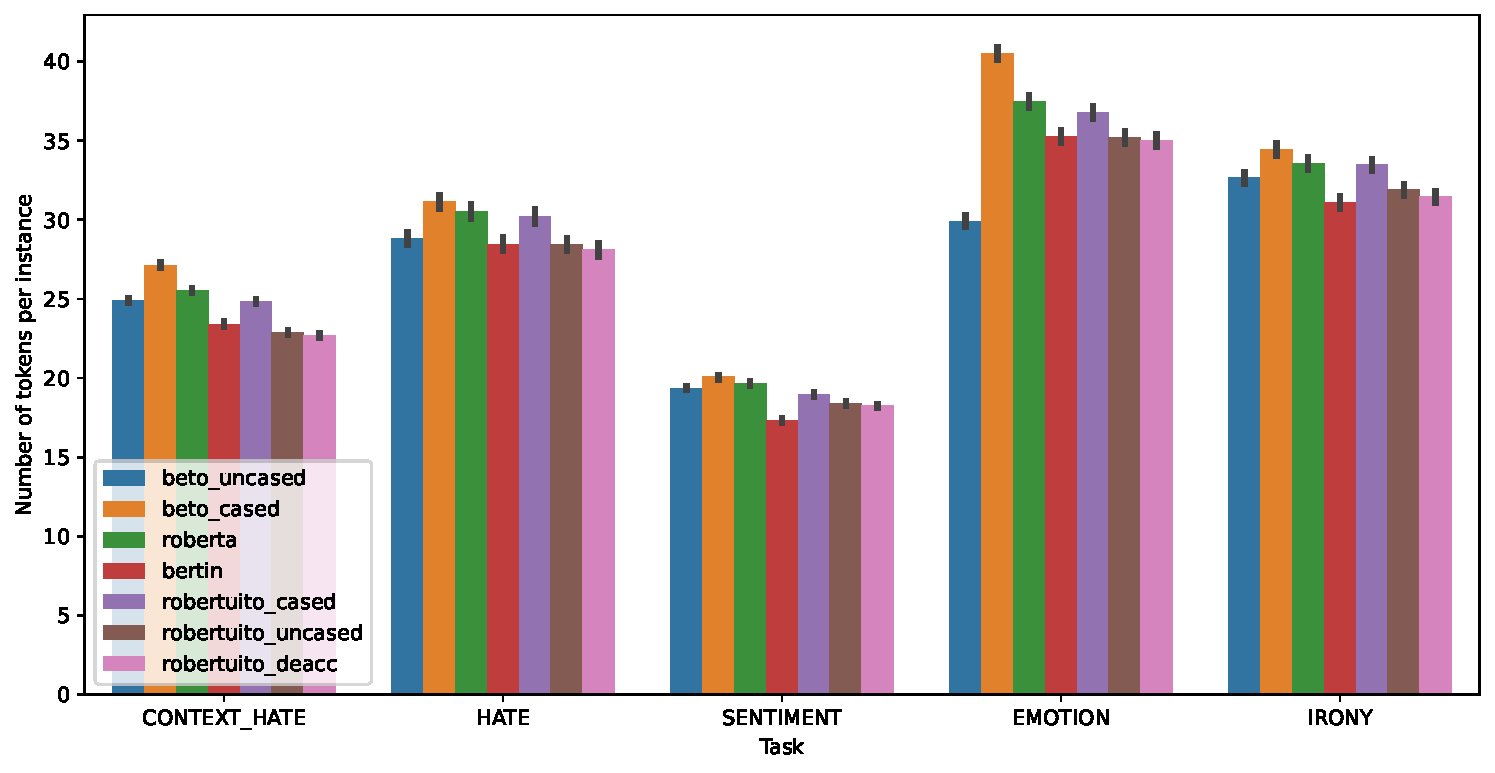
\includegraphics[width=\textwidth]{img/robertuito/length_tokens.pdf}
    \caption{Distribución de la cantidad de tokens por instancia para los tokenizadores de cada modelo. Las barras están agrupadas por tarea y muestran la media de la distribución junto a su intervalo de confianza a 95\%. Más chico es mejor.}
    \label{fig:length_tokens}
\end{figure}

La Figura \ref{fig:length_tokens} muestra la distribución del número de tokens en el texto de entrada agrupados por tarea. Podemos observar que los modelos de \robertuito{} tienen representaciones más compactas que \beto{} y \emph {RoBERTa-BNE}. \emph{BERTin}, a pesar de su menor rendimiento en general, tiene un tamaño medio comparable al de nuestro modelo. Entre los modelos de \robertuito{}, podemos observar que la versión \deacc{} tiene una longitud media ligeramente menor en comparación con la versión \uncased{}. En suma, esto indicaría que los modelos de \robertuito{} logran codificar de manera más eficiente los tweets de los distintos conjuntos de datos considerados.


\section{Adaptación de modelos pre-entrenados}
\label{sec:domain_adaptation_vs_robertuito}

Acabamos de observar que \robertuito{} obtiene una mejor performance que otros modelos pre-entrenados. Ahora, ¿puede ser esta mejora replicada adaptando otro modelo de lenguaje? Esta pregunta tiene --más allá del interés teórico de si un modelo de lenguaje entrenado en un dominio distinto puede adaptarse con éxito a un dominio diferente-- dos consideraciones prácticas: en lenguajes de recursos relativamente bajos, entrenar un modelo desde cero como realizamos en la anterior sección puede ser prohibitivo en términos de recursos \footnote{Con los recursos instalados de nuestro laboratorio es prácticamente imposible pre-entrenar un modelo desde cero}; y por otro lado, reducir los inmensos costos computacionales de entrenar puede ser de interés, tanto en términos económicos como ambientales.

Para contestar esta pregunta, realizamos una adaptación de dominio a un modelo BETO sobre textos generados por usuario --concretamente, los mismos datos usados para entrenar \robertuito{}-- y probamos su performance sobre el benchmark de tareas sociales descripto en la sección anterior.


\subsection{Metodología}

Para realizar la adaptación de dominio, seguimos las recomendaciones de \citet{gururangan-etal-2020-dont}: tomar un gran conjunto de datos no anotado de textos sociales, y correr la tarea de Masked Language-Modeling sobre estos. En términos de ese trabajo, estaríamos realizando \emph{Domain Adaptation Pre-training} (\emph{DAPT}), que consta de usar un conjunto de datos relativamente general. Para ello, utilizamos los mismos datos recolectados para entrenar a \robertuito{}.

Tomamos las versiones cased y uncased de BETO, y corrimos únicamente la tarea de MLM sobre estos datos. En lugar de correr por 12.5K pasos de optimización como es sugerido en este trabajo, probamos con 2.5K, 5K, 10K y 20K pasos de optimización, para analizar también el impacto de este hiperparámetro. Finalmente, nos quedamos con la configuración que obtuvo el mejor resultado en términos del benchmark analizado.

Para entrenar estos modelos, usamos una TPU v2-8, gracias también al programa TRC de Google. Cada paso de optimización tomó alrededor de 2.5 segundos. Usamos una configuración similar a la descripta para el entrenamiento de \robertuito{} (ver tabla \ref{tab:robertuito_architecture}), con un learning rate levemente superior ($5 * 10^-4$) y limitando también la longitud de secuencia a 128 tokens.

\subsection{Resultados}
\label{sec:domain_adaptation_results}


\begin{figure}
    \centering
    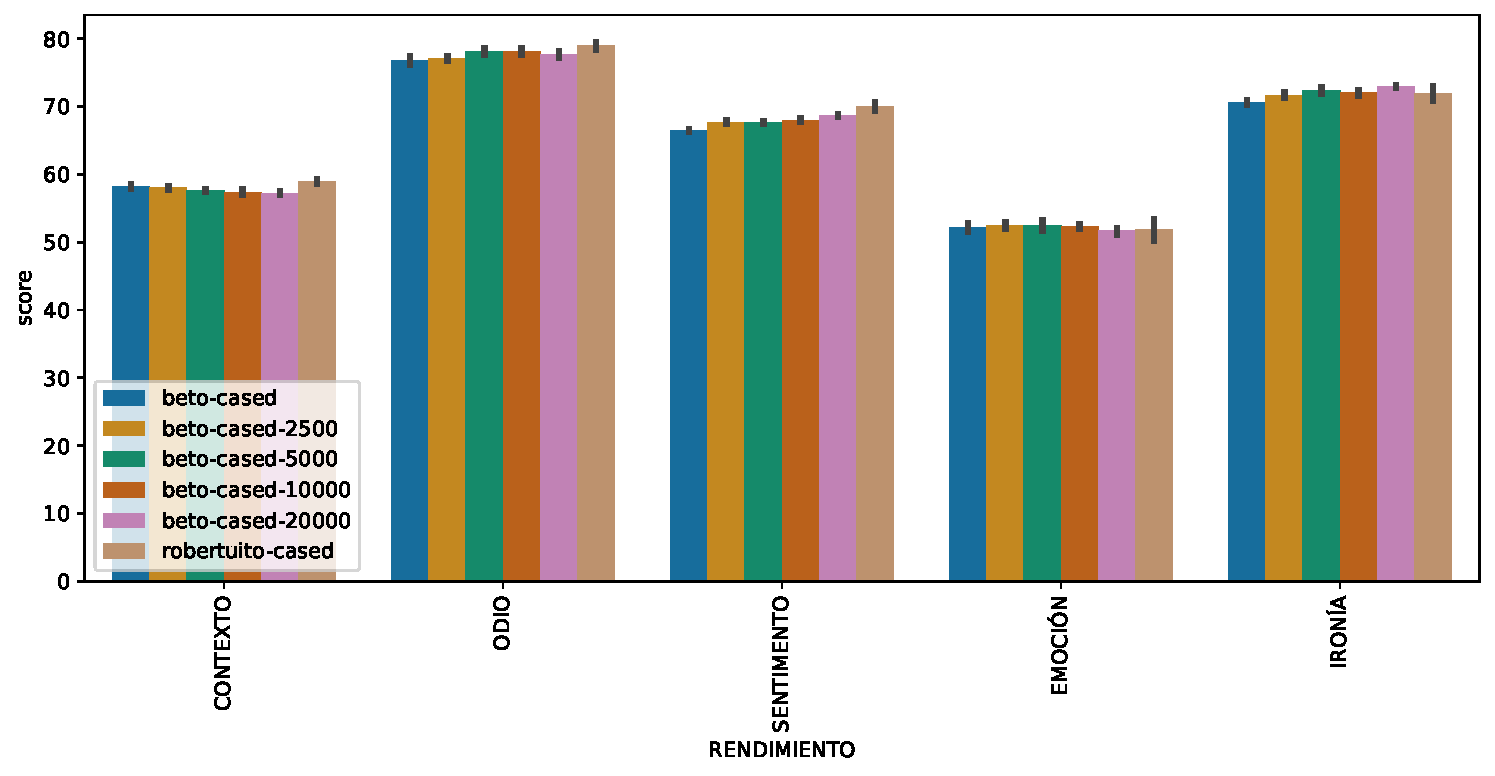
\includegraphics[width=\textwidth]{img/robertuito/results_cased_models.pdf}
    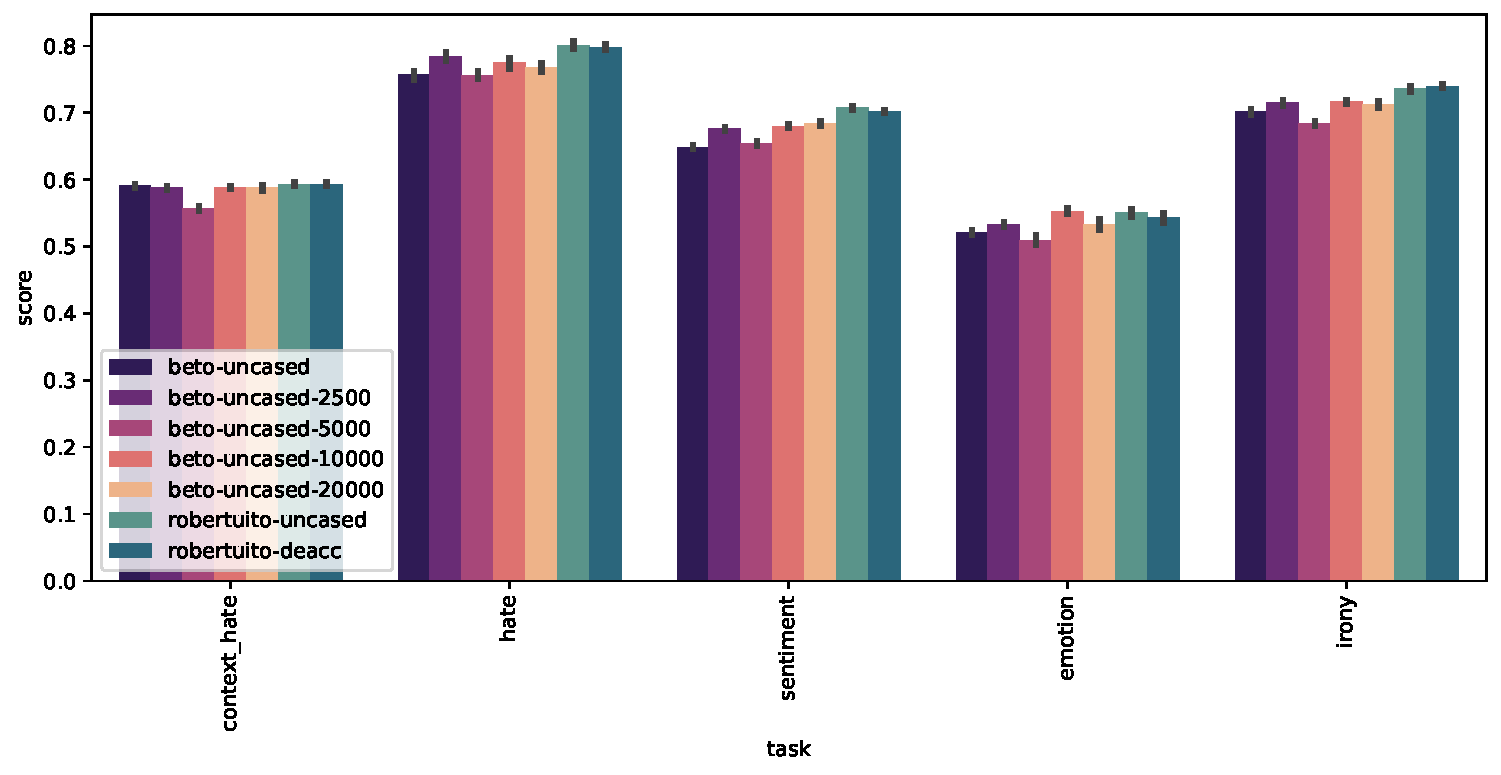
\includegraphics[width=\textwidth]{img/robertuito/results_uncased_models.pdf}

    \caption{Resultados sobre el benchmark de los modelos BETO y \robertuito{} (en versiones cased y uncased). Las barras están agrupadas por tarea y muestran la media de la performance sobre 15 corridas, junto a su intervalo 95\%. En tonalidad de rojo oscuro a amarillo están los modelos ajustados a dominio (más claro, más ajuste de dominio). El número al final de los modelos indica la cantidad de pasos de optimización realizados en el ajuste de dominio. En tonos azules las variantes de \robertuito{}}
    \label{fig:robertuito_vs_domain_barplot_results}
\end{figure}


En la figura \ref{fig:robertuito_vs_domain_barplot_results} podemos observar la performance para los modelos de lenguaje (\beto{} y \robertuito{}) así como también para las versiones con ajuste de dominio de \beto{}. Podemos observar que, para los modelos \emph{cased}, aumentar el pre-entrenamiento pareciera coincidir con una mejor performance; salvo para el caso de la tarea de detección de odio contextualizado. Una posible razón detrás de esto es que la tarea planteada tiene diferencias con el dominio sobre el cual ajustamos: utilizamos pares de tweets, uno de ellos (el contexto) proveniente de un medio periodístico. También puede argumentarse que el dominio de tweets en general es demasiado amplio \cite{eisenstein2013bad}.

En el caso de los modelos \emph{uncased}, esta mejora es un poco menos clara: por ejemplo, podemos observar que a los 5,000 pasos de optimización la performance sufre una caída con respecto a otras tareas. Esto puede deberse a problemas en la recolección de datos en los cuales entrenamos \robertuito{}, que se magnifican al realizar pocas actualizaciones. Sin embargo, salvando este caso puntual, observamos mejoras en todas las tareas, otra vez salvando el caso de la detección de odio contextualizada.



\begin{table}[ht]
    \centering
    \footnotesize
    \begin{tabular}{llllllr}
        \toprule
        Modelo             & CONTEXT                   &  HATE              &  SENTIMENT        &  EMOTION          &  IRONY            &     score \\
        \midrule
        beto-uncased       & $0.591 \pm 0.006$ & $0.757 \pm 0.012$ & $0.649 \pm 0.005$ & $0.521 \pm 0.006$& $0.702 \pm 0.008$& 0.644 \\
%       bertin             & $0.557 \pm 0.008$ & $0.767 \pm 0.005$ & $0.665 \pm 0.003$ & $0.518 \pm 0.012$& $0.716 \pm 0.008$& 0.644702 \\
        beto-cased         & $0.582 \pm 0.007$ & $0.768 \pm 0.012$ & $0.665 \pm 0.004$ & $0.521 \pm 0.012$& $0.706 \pm 0.007$& 0.648 \\
%       roberta-bne        & $0.577 \pm 0.004$ & $0.766 \pm 0.015$ & $0.669 \pm 0.006$ & $0.533 \pm 0.011$& $0.723 \pm 0.017$& 0.653565 \\
        beto-cased$_{FT}$   & $0.572 \pm 0.006$ & $0.777 \pm 0.009$ & $0.686 \pm 0.005$ & $0.517 \pm 0.009$& $0.730 \pm 0.004$& 0.656 \\
        beto-uncased$_{FT}$ & $0.588 \pm 0.003$ & $0.775 \pm 0.015$ & $0.680 \pm 0.004$ & $0.553 \pm 0.009$& $0.717 \pm 0.005$& 0.663 \\
        \hline
        robertuito-cased   & $0.590 \pm 0.005$ & $0.790 \pm 0.012$ & $0.701 \pm 0.012$ & $0.519 \pm 0.032$& $0.719 \pm 0.023$& 0.665 \\
        robertuito-deacc   & $0.593 \pm 0.006$ & $0.798 \pm 0.008$ & $0.702 \pm 0.004$ & $0.543 \pm 0.015$& $0.740 \pm 0.006$& 0.675 \\
        robertuito-uncased & $0.593 \pm 0.004$ & $0.801 \pm 0.010$ & $0.707 \pm 0.004$ & $0.551 \pm 0.011$& $0.736 \pm 0.008$& 0.678 \\
        \bottomrule
    \end{tabular}
    \caption{Resultados de la evaluación de modelos pre-entrenados y modelos ajustados en dominio para el benchmark de tareas sociales: CONTEXT es contextualized hate speech, HATE es hate speech detection sobre el dataset de hatEval, SENTIMENT, EMOTION e IRONY son análisis de sentimiento, emociones e ironía sobre los corpus de TASS. Todos los scores son Macro F1s. beto-cased-ft y beto-uncased-ft son modelos adaptados al dominio sociall. Score es la media de cada fila. }

    \label{tab:domain_adaptation_evaluation_results}

\end{table}

La tabla \ref{tab:domain_adaptation_evaluation_results} muestra las medias de los resultados junto a sus desviaciones estándar para los modelos \emph{uncased}, que tienen los mejores resultados (ver en apéndice \ref{app:07} la tabla completa). Seleccionamos como modelos ajustados a dominio (indicados con el subíndice $FT$) a aquellos modelos que obtuvieron una mejor performance entre aquellos que entrenamos con distinta cantidad de pasos de optimización. Haciendo una comparación entre los modelos \beto{} y \robertuito{} uncased, vemos en el caso de la tarea de HatEval que el gap es de alrededor de 4.4 puntos de F1, mientras que la versión FT achica esa diferencia a 2.26 puntos F1, una reducción del 48\% del gap de performance. En el caso de Sentiment Analysis, pasamos de un gap de 5.8 puntos de F1 a uno de 2.7, una achicando en un 53\% la diferencia de performances. En el caso de Emotion Analysis, este gap pasa de 3 puntos de F1 a 0, de hecho logrando mejores resultados. Finalmente, en el caso de detección de ironía, el gap de 3.4 puntos de F1 pasa a 1.9, una reducción de 44\%.




\section{Discusión}

En primer lugar, \robertuito{} presenta mejoras significativas para casi todas las tareas, con picos de hasta casi 4 puntos de F1 para la tarea de Sentiment Analysis contra le mejor versión de \beto{}. La mejora es muy marginal en el caso de la tarea del dataset construído en el capítulo \ref{chap:05_dataset_creation}, y no pareciera ser significativa. Esto puede deberse a que este dataset tiene una estructura bastante diferente de la de las otras tareas: cada instancia es una composición de dos tweets, uno de los cuales (el contexto) es en la mayoría de los casos un titular de diarios (formulado como un tweet), y por otro lado el comentario efectivo que se analiza como discurso de odio. Esto puede mitigar las potenciales mejoras de \robertuito{} por dos razones: el dominio del contexto no es demasiado distinto que el dominio de entrenamiento de BETO, y el tipo de pre-entrenamiento sólo con MLM y no en pares de tweets (recordemos que sólo hacemos MLM y no Next-Sentence Prediction). Sobre la segunda posible razón, podemos observar (para la tarea de detección de discurso de odio contextualizado) que los modelos con pre-entrenamiento basado en RoBERTa (\emph{roberta-bne} y \emph{bertin}) tienen peor performance que las dos versiones de \emph{BETO}.

De los distintos tipos de normalización de texto utilizados en \robertuito{} (\emph{cased}, \emph{uncased} y \emph{deacc}), podemos observar que los modelos \emph{uncased} y \emph{deacc} obtienen mejores performances en general. Si bien el modelo \emph{uncased} muestra una ligera performance superior al modelo \emph{deacc}, esta mejora no es significativa, y esto indicaría que remover tildes no reporta una degradación de la performance. Esto es esperable ya que usualmente no se utiliza esta marcación en el español ``vulgar'' utilizado en las redes sociales. Sin embargo, para llegar a esta conclusión sería necesario realizar pruebas más extensivas sobre otras tareas y verificando el correcto pre-entrenamiento de estos modelos.

Con respecto a los experimentos de adaptación de dominio, podemos observar que adaptando BETO obtenemos una mejora en todos las tareas contra la versión no ajustada. Comparado con \robertuito{}, las versiones a las que les realizamos fine-tuning logran recortar alrededor del 50\% del performance gap entre \robertuito{} y BETO; en algunos casos, incluso reduciéndolo a 0. Esta comparación, sin embargo, no es del todo justa ya que BETO fue entrenado de una manera distinta que \robertuito{}. Por cuestiones de tiempo no pudieron ser realizados sobre \emph{roberta-bne}(principalmente, ya que éste modelo y \emph{bertin} fueron lanzados mientras hacíamos estos experimentos) pero debería esto ser verificado en el futuro. Puede que este gap sea reducido aún más partiendo desde este otro modelo, y analizando algunas otras opciones que no tratamos en este capítulo: por ejemplo, agregar vocabulario en el ajuste de dominio, algo que por ejemplo la librería \emph{fastai} realiza en su implementación de ULM-FIT.

Una consideración práctica de la adaptación de dominio es que permite, en lugar de realizar un costo pre-entrenamiento desde cero (como en el caso de MedBERT y SciBERT que ya relatamos anteriormente), mejorar la performance de un modelo de lenguaje ya entrenado de una manera relativamente económica. En términos concretos, un ajuste de dominio puede realizarse utilizando una placa de GPU en uno o dos días de entrenamiento, mientras que pre-entrenar un modelo desde cero requiere acceso a un hardware más oneroso. Algunos trabajos recientes \cite{izsak2021train} muestran alternativas para hacer esto con recursos reducidos ajustando varios hiperparámetros y usando algunas técnicas de optimización reciente (como LAMB \cite{you2019large}); sin embargo, muchos de estos setups están lejos del alcance de los recursos disponibles de muchos laboratorios. En este escenario, aplicar una optimización de dominio aparece como una alternativa mucho más factible.

Una de las limitaciones de lo estudiado es que \robertuito{} fue entrenado sólo por 600k pasos de optimización, contra los casi 900k pasos de \beto{}, y los 1M de \bertweet{}. Hay que observar, que la optimización de \beto{} se da con un batch size menor (512 vs 4k que usa \robertuito{}) y la de \bertweet{} se hace un batch size mayor (7k). En el caso de los modelos basados en \roberta{} en español, no tenemos disponible esa información. Con lo cual, esta comparación no es totalmente justa. Otra limitación es la escasa disponibilidad de tareas en español para textos sociales por fuera de clasificación: en \citet{bertweet}, por ejemplo, se estudian también problemas de POS tagging y de NER para textos sociales en inglés.

\section{Conclusiones}

En este capítulo, hemos abordado la tarea de mejorar la performance de la detección de discurso de odio para las tareas planteadas en esta tesis y en el contexto más general de tareas de clasificación sobre textos sociales en español. Para ello, utilizamos como benchmark varias de las tareas que vimos en esta tesis: detección de discurso de odio (en sus dos versiones, no contextualizada y contextualizada), análisis de sentimiento, análisis de emociones, y detección de ironía.

En primer lugar, y en la corriente de modelos pre-entrenados sobre distintos dominios, generamos un nuevo y valioso recurso para la clasificación de textos sociales: \robertuito{}, un modelo de lenguaje basado en \roberta{} sobre tweets en español. Para ello, recolectamos una gran base de datos de tweets en español, y utilizando las TPU provistas por Google realizamos el pre-entrenamiento de este modelo. Los experimentos de clasificación sobre el benchmark arrojaron que \robertuito{} obtiene mejores significativas sobre otros modelos en español. Así mismo, observamos que remover tildes en el preprocesado no reporta una degradación significativa en la performance.

Por otro lado, exploramos un ajuste de dominio sobre modelos actuales para comparar la ganancia de performance y compararla contra \robertuito{}. Para ello, tomamos los modelos de \beto{} (en sus versiones cased y uncased) y corrimos la tarea de MLM sobre los tweets recolectados para entrenar nuestro modelo anterior. Si bien la performance de estos modelos ajustados mejora con respecto de \beto{}, se mantiene por debajo de \robertuito{}, aunque recortando considerablemente el gap de performance entre ambos modelos. De todas formas, este análisis puede ser de consideración para aquellos lenguajes con menos recursos que no pueden pre-entrenar modelos de lenguaje desde cero. Resta como trabajo futuro realizar estos experimentos sobre más tareas más ricas que no sean exclusivamente de clasificación, y realizar los ajustes sobre los modelos \roberta{} en español para hacer una comparación más justa.

Todos estos experimentos han sido realizados en español. Publicamos tanto el modelo \robertuito{}(\footnote{\url{https://huggingface.co/finiteautomata/robertuito-base-uncased}}), el código para entrenarlo y para correr el benchmark con otros modelos pre-entrenados \footnote{Ambos en  \footnote{\url{https://github.com/pysentimiento/robertuito}}}  y la base de datos de tweets en español.

\section{Notas}

En \citet{perez2021robertuito} puede encontrarse la descripción de la construcción de \robertuito{}, aproximadamente la mitad de este capítulo. En el apéndice \ref{app:07} puede encontrarse la tabla completa de resultados para las distintas cantidades de pasos de optimización.

